
%================================
\subsection{Pruebas con OpenMP con optimización por compilador}
\label{sec:Pruebas con OpenMP con optimizacion por compilador}


\subsubsection{Pruebas con 2 hilos}
\label{sec:Pruebas con 2 hilos optimizado}

\begin{table}[H]
   \centering
   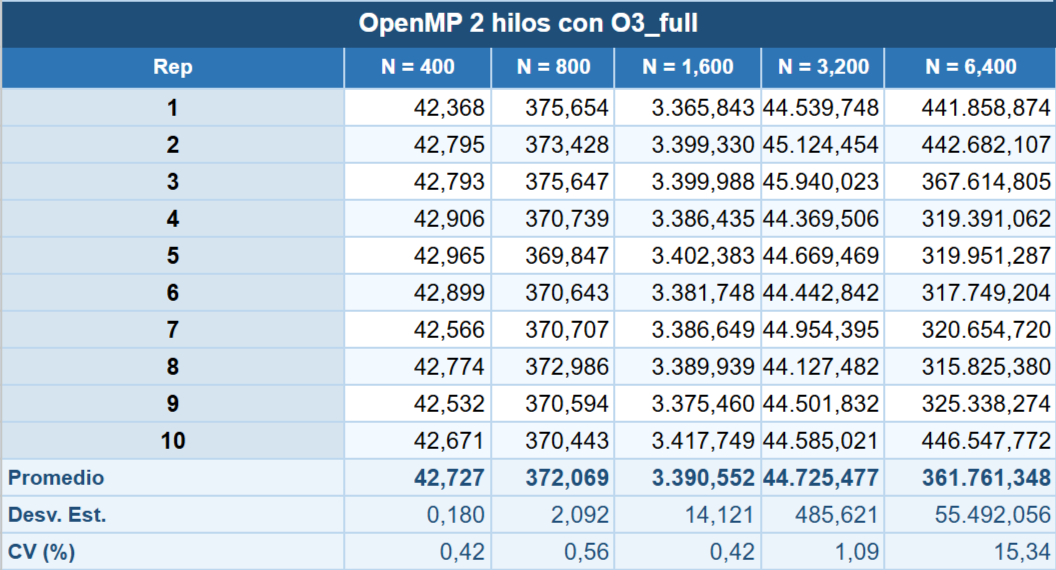
\includegraphics[width=1\textwidth]{images/omp/tables/time_machine1_2t_opt.png}
   \caption{Resultados de tiempo para la multiplicación de matrices utilizando OpenMP con 2 hilos}
   \label{tab:time_machine1_2_threads_opt}
\end{table}


\subsubsection{Pruebas con 4 hilos}
\label{sec:Pruebas con 4 hilos optimizado}

\begin{table}[H]
   \centering
   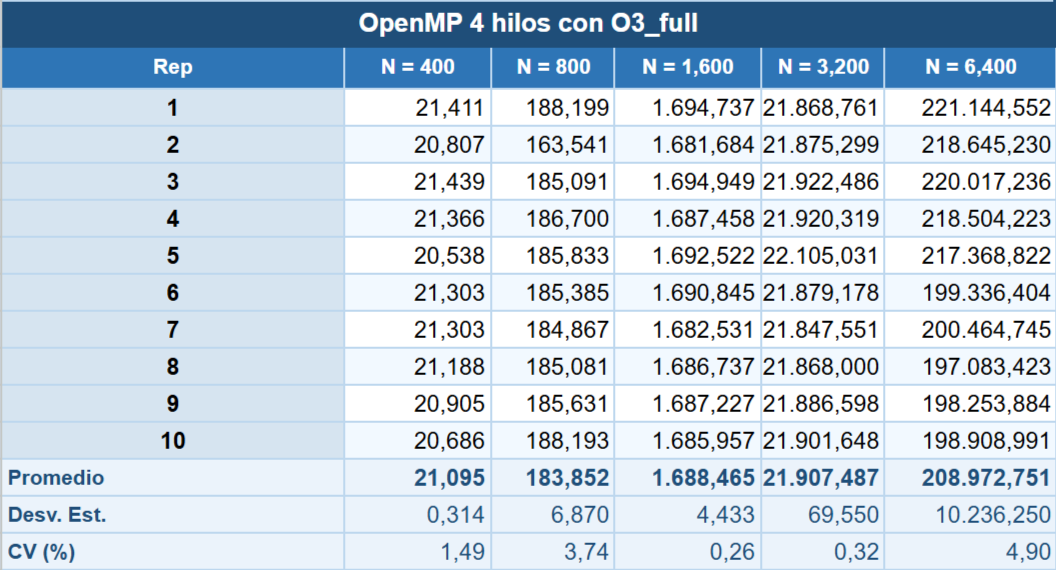
\includegraphics[width=1\textwidth]{images/omp/tables/time_machine1_4t_opt.png}
   \caption{Resultados de tiempo para la multiplicación de matrices utilizando OpenMP con 4 hilos}
   \label{tab:time_machine1_4_threads_opt}
\end{table}


%================================
\subsubsection{Pruebas con 6 hilos}
\label{sec:Pruebas con 6 hilos optimizado}

\begin{table}[H]
   \centering
   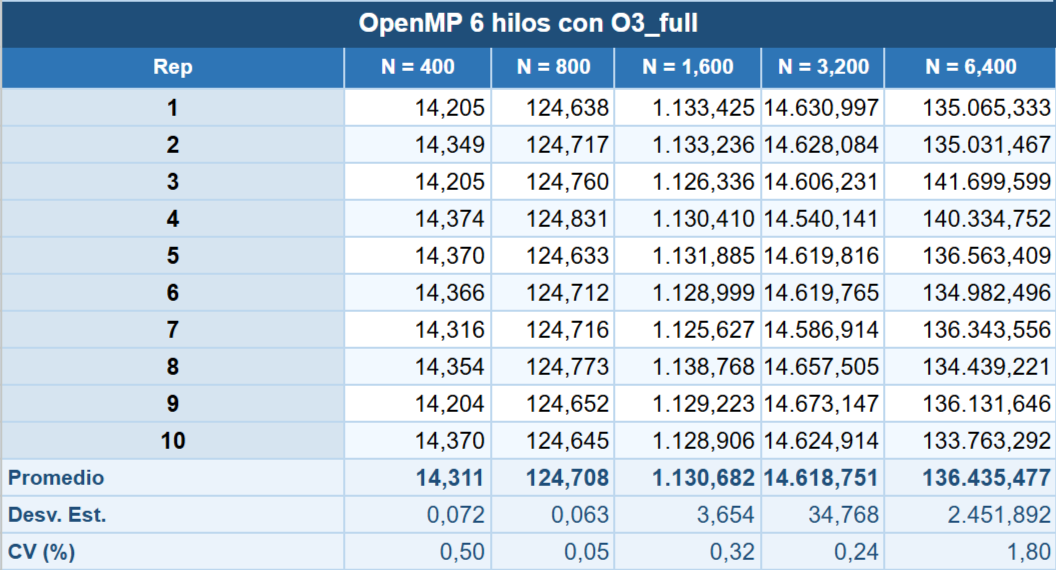
\includegraphics[width=1\textwidth]{images/omp/tables/time_machine1_6t_opt.png}
   \caption{Resultados de tiempo para la multiplicación de matrices utilizando OpenMP con 6 hilos}
   \label{tab:time_machine1_6_threads_opt}
\end{table}


\subsubsection{Pruebas con 8 hilos} 
\label{sec:Pruebas con 8 hilos optimizado}

\begin{table}[H]
   \centering
   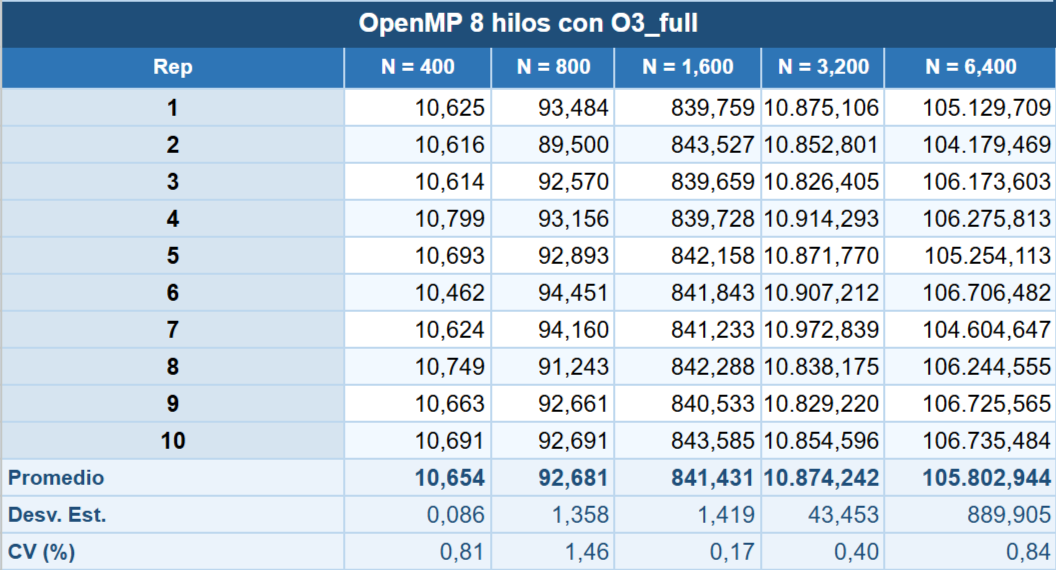
\includegraphics[width=1\textwidth]{images/omp/tables/time_machine1_8t_opt.png}
   \caption{Resultados de tiempo para la multiplicación de matrices utilizando OpenMP con 8 hilos}
   \label{tab:time_machine1_8_threads_opt}
\end{table}

\subsubsection{Pruebas con 12 hilos}
\label{sec:Pruebas con 12 hilos optimizado}

\begin{table}[H]
   \centering
   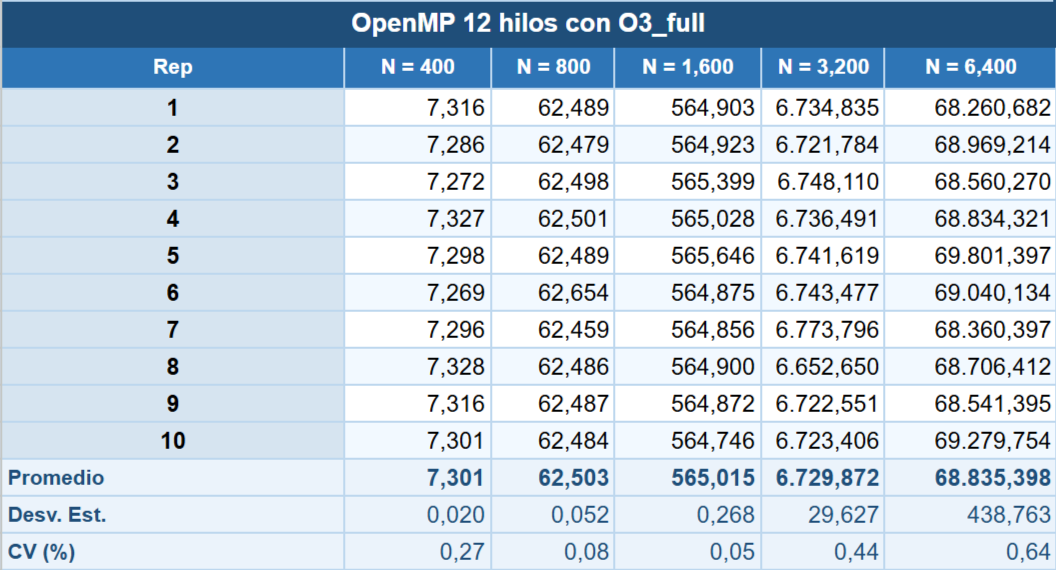
\includegraphics[width=1\textwidth]{images/omp/tables/time_machine1_12t_opt.png}
   \caption{Resultados de tiempo para la multiplicación de matrices utilizando OpenMP con 12 hilos}
   \label{tab:time_machine1_12_threads_opt}
\end{table}



%================================
\subsubsection{Gráfica de tiempo}
\label{sec:Grafica de tiempo}

\begin{figure}[H]
   \centering
   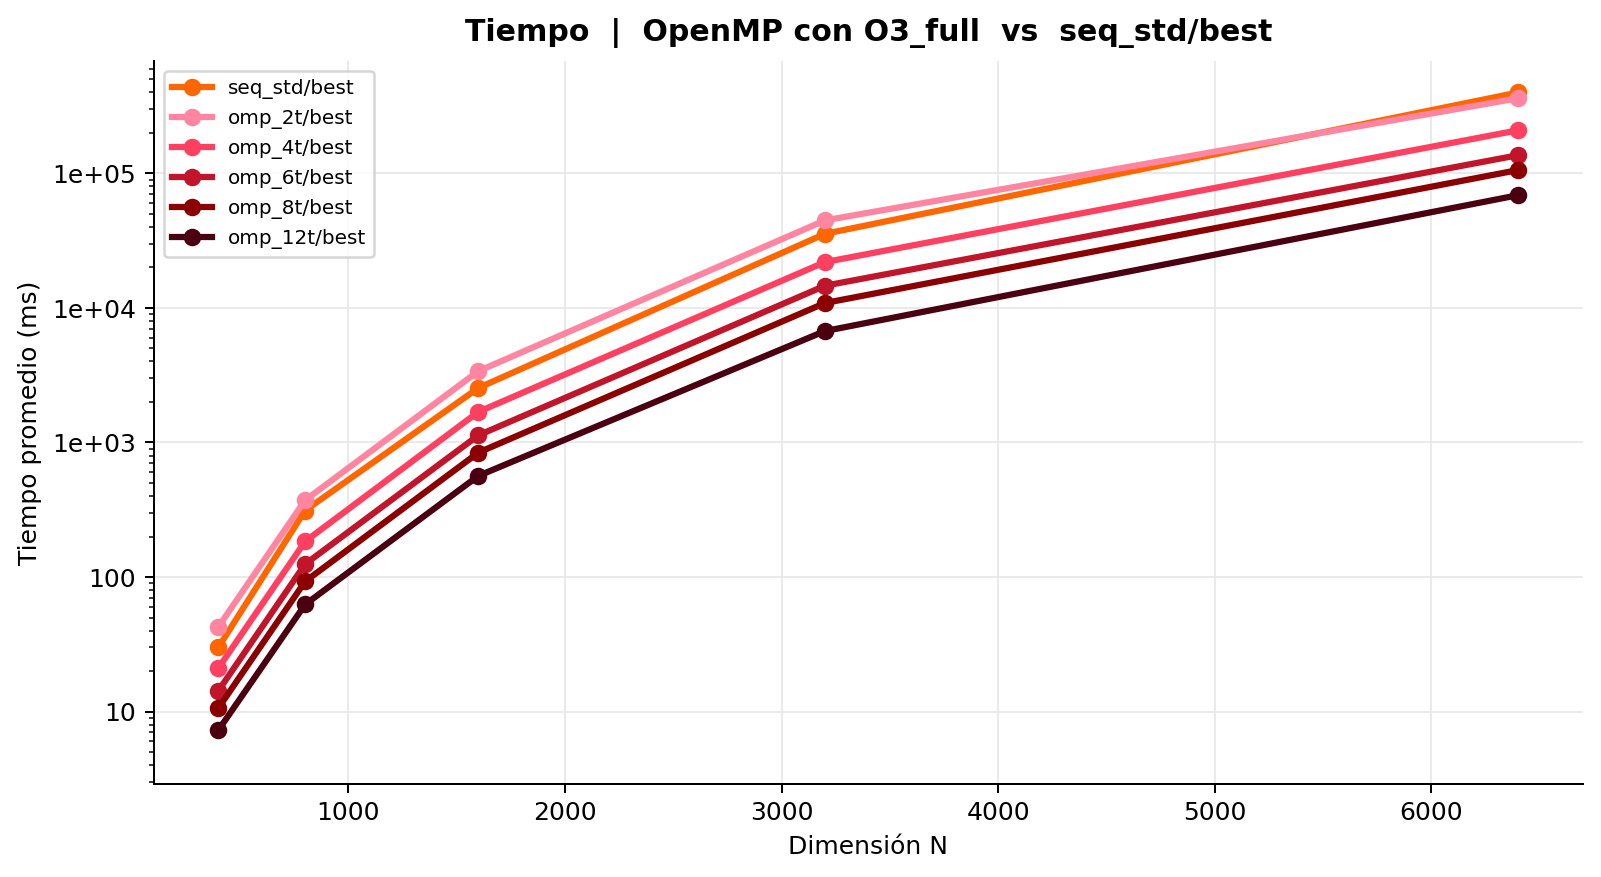
\includegraphics[width=1\textwidth]{images/omp/charts/time_opt.png}
   \caption{Gráfica de tiempo para la multiplicación de matrices utilizando OpenMP con optimización por compilador}
\end{figure}


%================================
\subsubsection{Speedup con OpenMP con optimización}
\label{sec:Speedup con OpenMP optimizado}

\begin{table}[H]
   \centering
   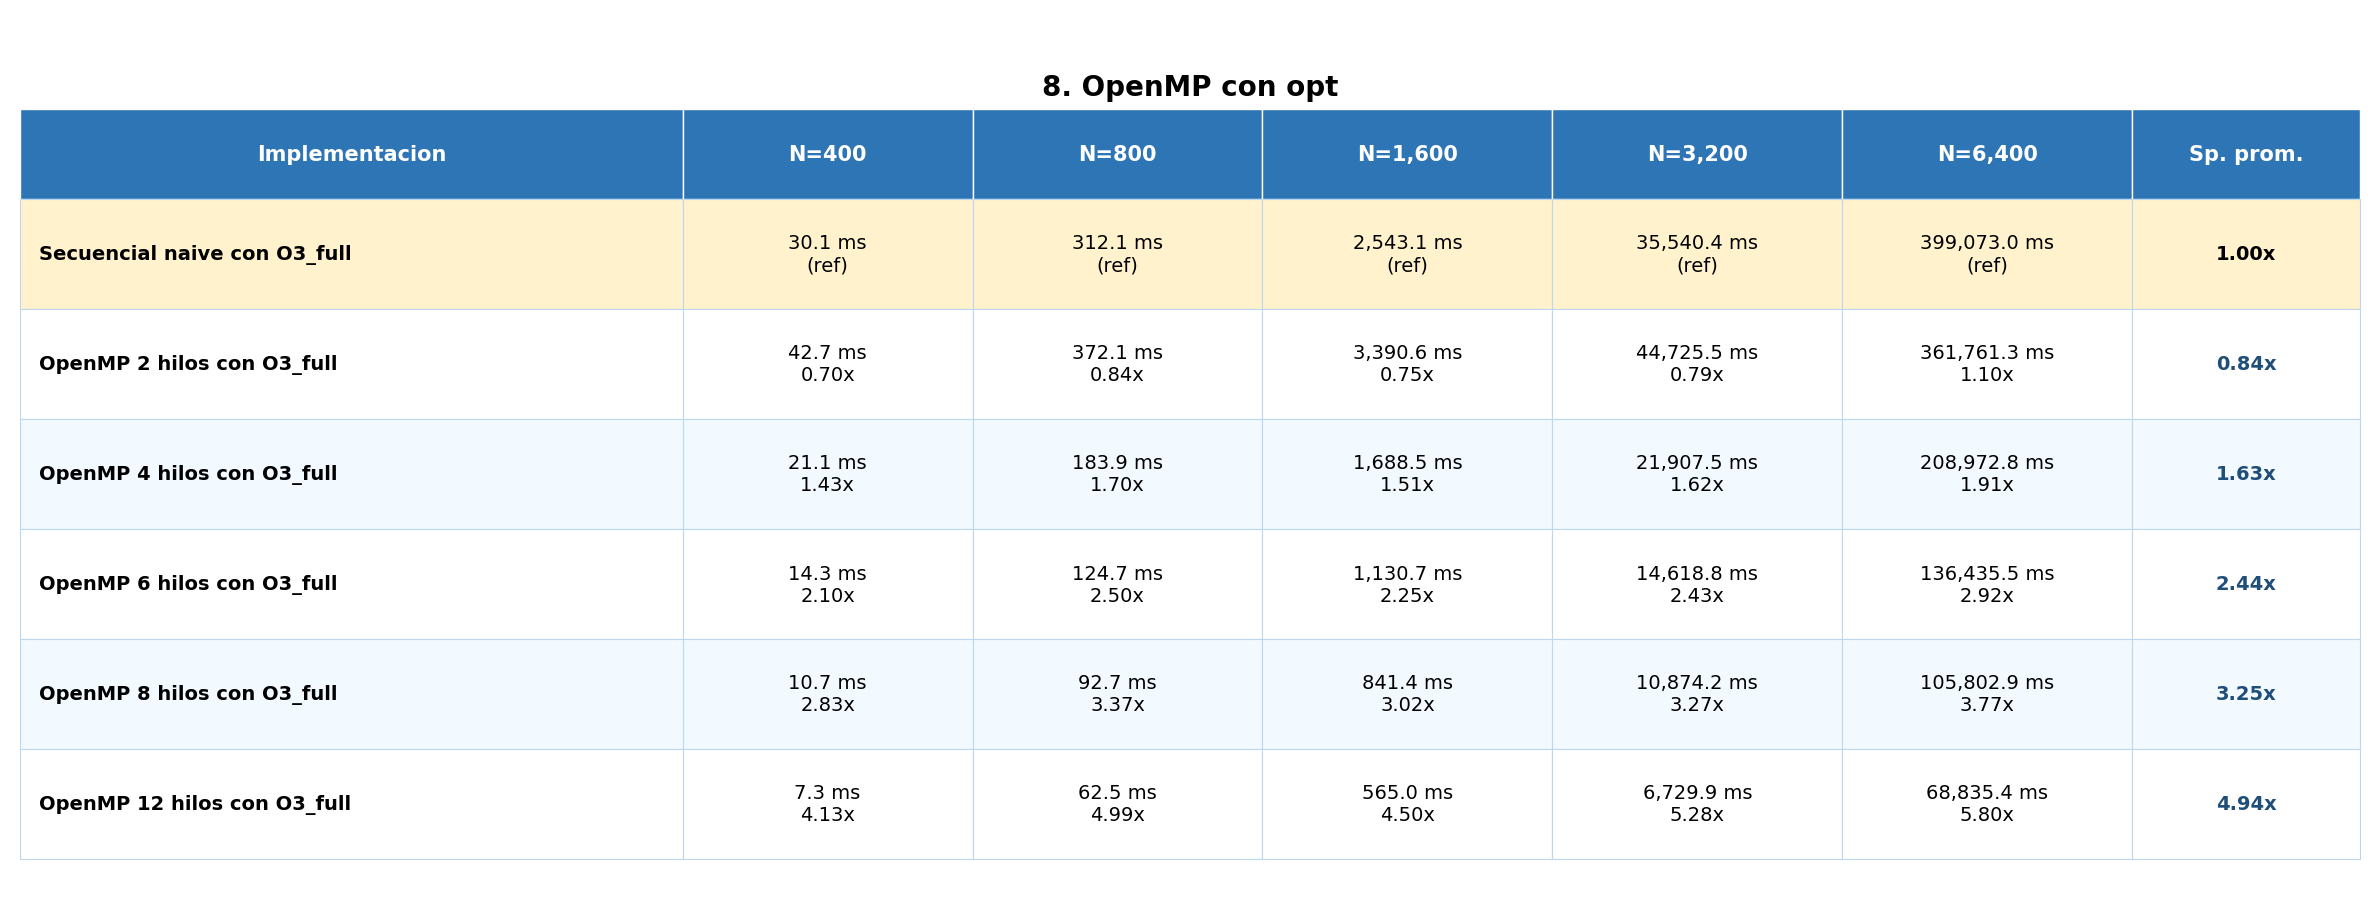
\includegraphics[width=1\textwidth]{images/omp/tables/table_opt_speedup.png}
   \caption{Resultados de Speedup para la multiplicación de matrices utilizando OpenMP con optimización por compilador}
   \label{tab:speedup_machine1_opt}
\end{table}

\begin{figure}[H]
   \centering
   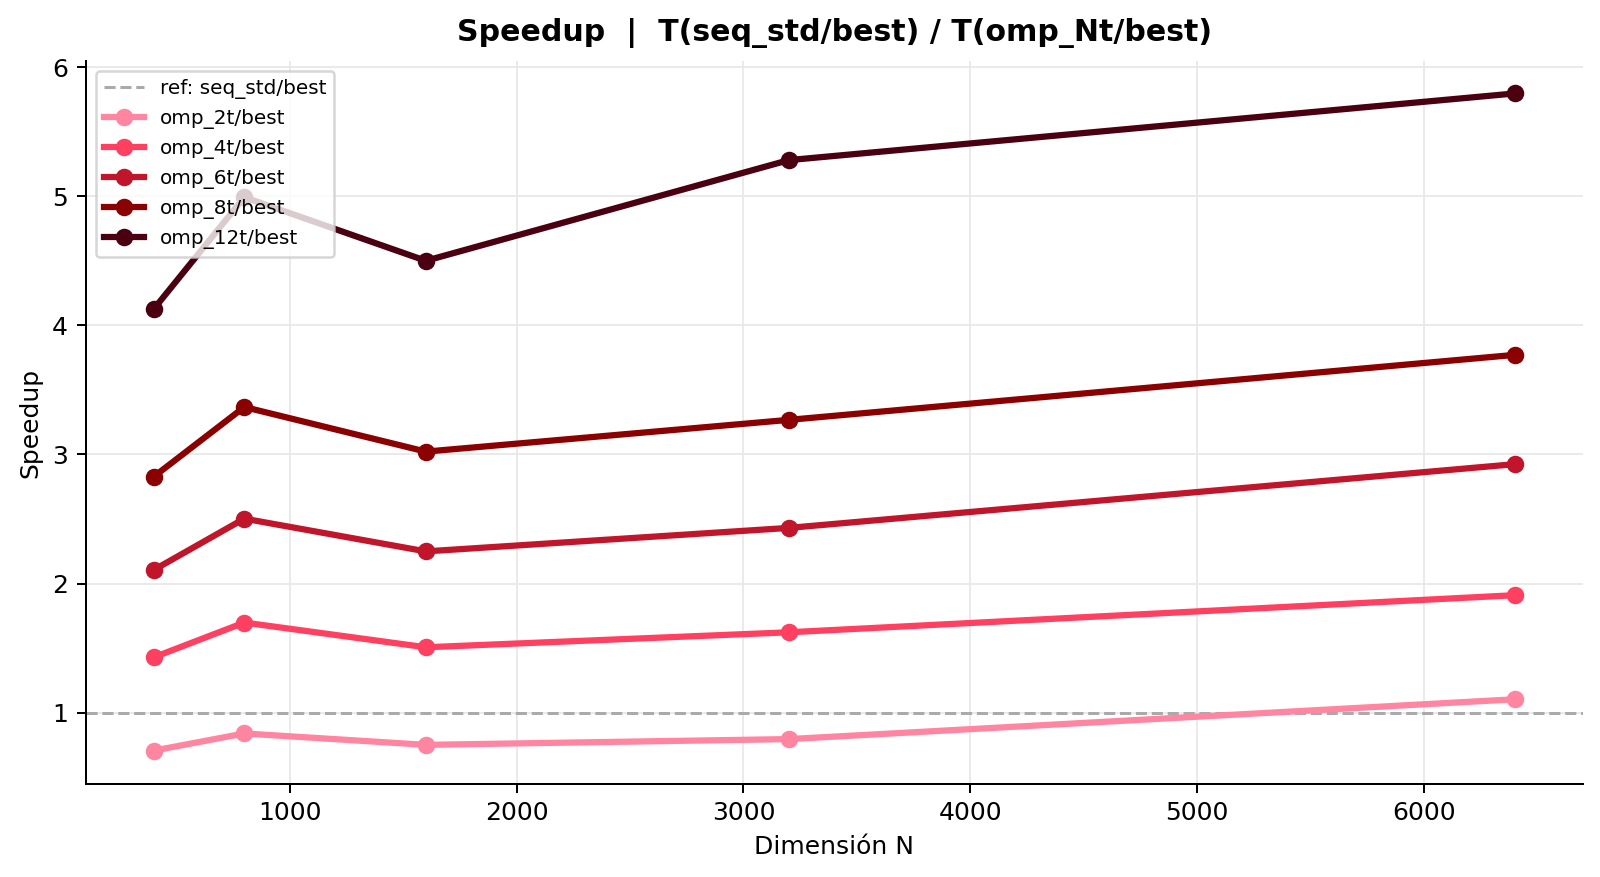
\includegraphics[width=1\textwidth]{images/omp/charts/speedup_opt.png}
   \caption{Gráfica de Speedup para la multiplicación de matrices utilizando OpenMP con optimización}
\end{figure}

En este caso, vemos una mejora significativa en el tiempo de ejecución al utilizar la optimización por compilador, especialmente a medida que se incrementa el número de hilos. El speedup también muestra una mejora considerable, alcanzando un máximo de 4.94x con 12 hilos, lo que indica que la optimización por compilador ha permitido aprovechar mejor los recursos del sistema y reducir el overhead asociado con la paralelización.